\documentclass[11pt]{article}
\usepackage{ucs}
\usepackage[utf8x]{inputenc}
\usepackage{geometry}
\usepackage[greek,english]{babel}
\newcommand{\en}{\selectlanguage{english}}
\newcommand{\gr}{\selectlanguage{greek}}
\usepackage{amsmath}
\usepackage{amssymb}
\usepackage{mathtools}
\usepackage{float}
\usepackage{graphicx}
\usepackage{a4wide}


\usepackage{tikz}
\usepackage{titlesec}
\usepackage{caption}
\setcounter{secnumdepth}{4}
\usepackage[bottom]{footmisc}

\usepackage{xcolor} % colors
\usepackage[toc,page]{appendix} % for appendices
\usepackage{csquotes} % for quotes
\usepackage{cancel} % for canceling values to zero

\allowdisplaybreaks % allows split between pages

\DeclarePairedDelimiter{\ceil}{\lceil}{\rceil}
\DeclarePairedDelimiter\floor{\lfloor}{\rfloor}
\usepackage{wrapfig} % wrap text to figure


%\usepackage{fancyhdr} % for header
%\pagestyle{fancy}
%\fancyhf{}
%\fancyfoot[C]{\thepage} % centere number of page
%%\fancyhead[R]{\rightmark}
\usepackage{bm} % BOLD

\usepackage{listings}

\usepackage{caption}
\usepackage{subcaption}
%\usepackage{algorithmic} % for algorithms
\usepackage[ruled,vlined]{algorithm2e}

\newcommand{\approxtext}[1]{\ensuremath{\stackrel{\text{#1}}{\approx}}}
%\renewcommand{\footrulewidth}{0.4pt}% default is 0pt

\usepackage[framed]{matlab-prettifier}
\newcommand\numberthis{\addtocounter{equation}{1}\tag{\theequation}}
\renewcommand{\lstlistingname}{Code}


\usepackage{optidef}
\usepackage{hyperref}
\usepackage{enumitem}

\hypersetup{
	colorlinks   = true, %Colours links instead of ugly boxes
	urlcolor     = blue, %Colour for external hyperlinks
	linkcolor    = blue, %Colour of internal links
	citecolor   = red %Colour of citations
}

\setlength{\parskip}{1em}
\DeclareMathOperator*{\argmax}{argmax} % FOR ARGMAX
\DeclareMathOperator*{\argmin}{argmin} % FOR ARGMIN
\DeclareMathOperator{\tr}{tr}
\DeclareMathOperator{\mean}{E}
\DeclareMathOperator{\rank}{rank}
\DeclareMathOperator{\diag}{diag}
\DeclareMathOperator{\sgn}{sgn}

\begin{document}
	\begin{titlepage}
		\title{\hrulefill\\
			\vspace{5mm}
			{\Huge \textbf{K-Means clustering algorithm in MapReduce}} \\ \hrulefill\\
			\vspace{10mm}
			{\Large {{Assignment 2}
		}}}
		\author{Panourgia Evangelia (t8190130)\\
			Papadatos Iwannis (t8190314)\\
			Professor: Damianos Chatziantwniou}
		\date{Latest Update: \today}
		\maketitle
		
		\thispagestyle{empty}
		\begin{center}
			
\includegraphics[width=0.3\textwidth]{./aueblogo.jpg}\\
			\vspace{10mm}
			School of Management Science and Technology,\\ Athens University of Economics and Business
		\end{center}
	\end{titlepage}
	\noindent
	
	\tableofcontents	
	
	\section{Hadoop Installation}
	As far as the installation of Hadoop, we decided to download Hadoop packaged by Bitnami [1] and Oracle VirtualBox[2].  When the package for Hadoop was downloaded, we import it to  Oracle VirtualBox and run it. After, these steps you can see in your pc the image shows in fig. 1. We note that as default username, password is the word bitname(look red letters). 
	Now, you should set the scene by installing git[2] (command : sudo apt-get install git), pip3(sudo apt install python3-pip)[3] and mrjob(pip3 install mrjob)[4]. So, now you have the necessary tools - software so as to run the code. 
    

	\begin{figure}[H]
		\makebox[\textwidth][c]{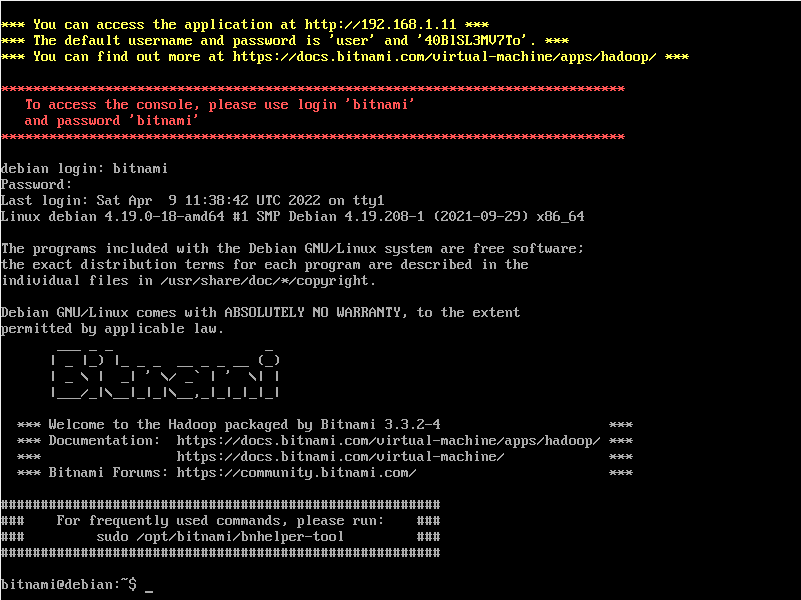
\includegraphics[width=.7\textwidth]{figs/img/install_bitnami.png}}
		\caption{Install Bitnami}
	\end{figure}

	
	\newpage
	\section{Dataset Creation}
	The file dataGenerate.py was written for generating data - points in the form (x, y). Specifically, it reads data from file centroids.csv which contains three centroids in the form (x, y) and then generate 8000 data points using python library skewnorm[5]. Last but not least, user can see the the generated data graphically by entering python3 generateData.py -d, ehere -d parameters call suitable function to draw[6] data points(see fig 2.).
	        
	
	\begin{figure}[H]
		\makebox[\textwidth][c]{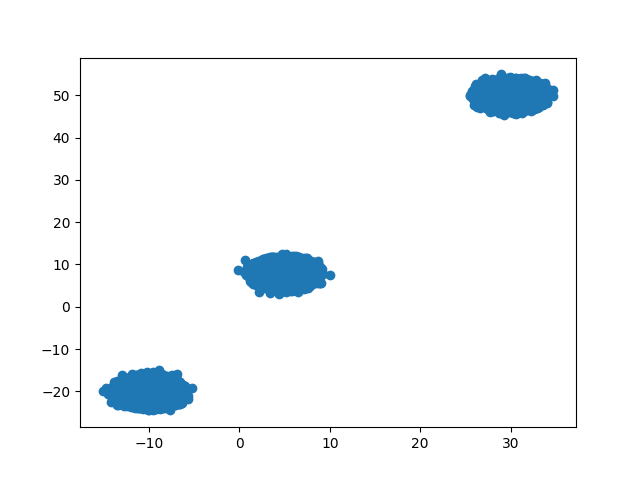
\includegraphics[width=.7\textwidth]{figs/img/plot.png}}
		\caption{Dataset Creation}
	\end{figure}
	
Now, we can see the code for data generation. 

	
	
	\newpage
	\section{K-Means Clustering Algorithm}
	
	The file kmeans.py was written to implement the algorithm kmeans[6] using MapReduce. For this aim, we used the python library mrjob. Firstly, we defined configuration and steps. Then, we write the function for mapper and reducer. For mapper, we calculate euclidean distance and for each point (x, y) we calculate all distances from all centroids and we hold the minimum distance, so we assign point to suitable centroid. Last but not least, the only work of reducer is to revise cluster centers as mean of assigned observations.
	
	Now, we can see the code for kmeans implementation. 
	
	\begin{figure}[H]
		\makebox[\textwidth][c]{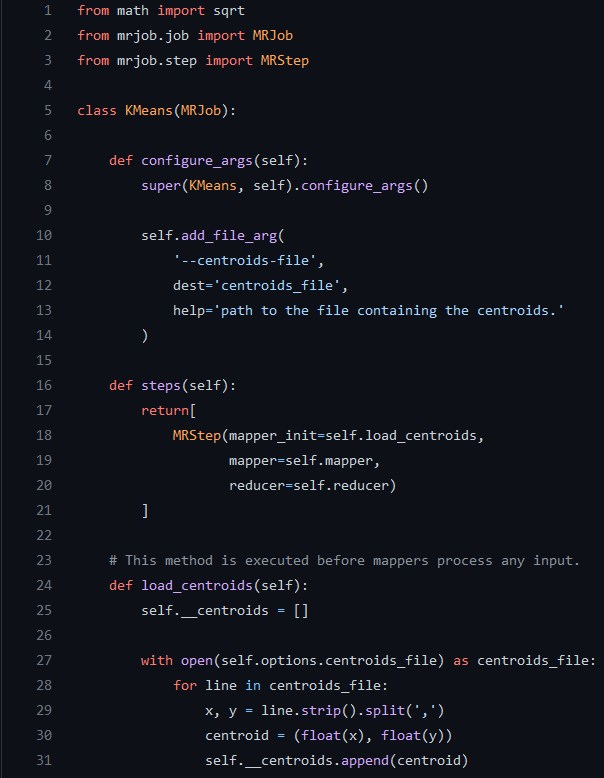
\includegraphics[width=.7\textwidth]{figs/img/kmeans_1.png}}
		\caption{kmeans implementation}
	\end{figure}
	
	\begin{figure}[H]
		\makebox[\textwidth][c]{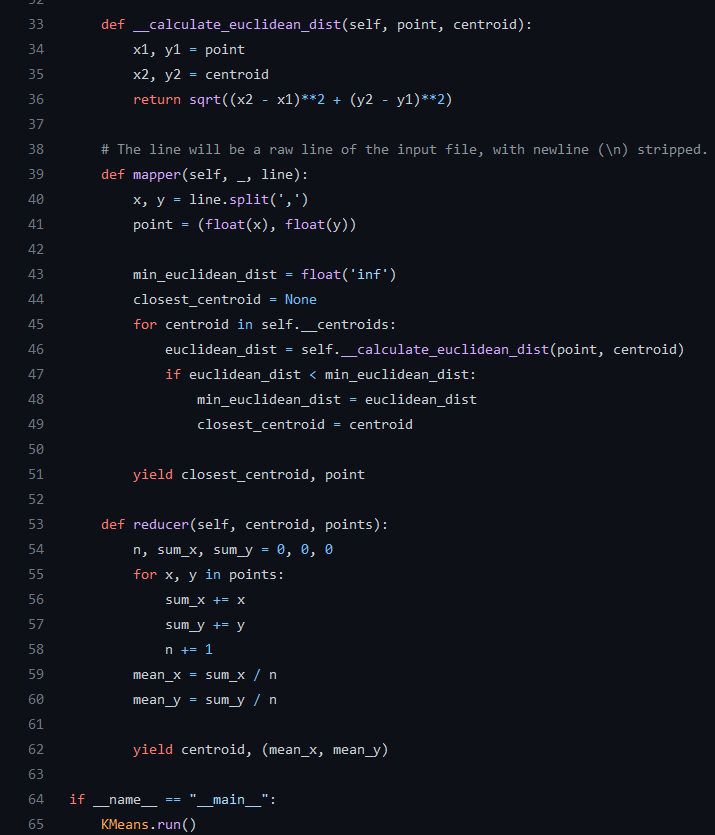
\includegraphics[width=.7\textwidth]{figs/img/kmeans_2.png}}
		\caption{kmeans implementation}
	\end{figure}
	
	\subsection{HDFS}   

	\subsection{Run}
	So, git clone + commands 
	

	\begin{thebibliography}{1}
		\bibitem{beck}
		Hadoop packaged by Bitnami, \textit{\textbf{https://bitnami.com/stack/hadoop/virtual-machine}}
	
	
		\bibitem{beck}
		Oracle VirtualBox, \textit{\textbf{https://www.virtualbox.org/}}
		
		\bibitem{beck}
		Install pip3, \textit{\textbf{https://linuxize.com/post/how-to-install-pip-on-ubuntu-18.04/}}
		
		\bibitem{beck}
		Install mrjob, \textit{\textbf{https://pypi.org/project/mrjob/}}
		
		\bibitem{beck}
		skewnorm, \textit{\textbf{https://docs.scipy.org/doc/scipy/reference/generated/scipy.stats.skewnorm.html}}
		
		\bibitem{beck}
		matplotlib, \textit{\textbf{https://matplotlib.org/}}
		
		
	\end{thebibliography}
	
	
\end{document}